\section{Purpose and Scope}
  Nowadays there are various sources of information.

  Light sources, such as RenRen, Sina Micro Blog (Weibo) produce news all the time.
  Many users are using one, or all, of them, then they need to open one or more webpages in order to get all the news feeds.

  Moreover, some heavey sources like NetEase, Yahoo!, or some other individual blogs may produce information from time to time.
  Readers may not be willing to refresh them again and again to get the latest article.

  Therefore, an information collector is in great demand, in order to simplify the flow of getting the latest information.
  Users can find what they want in just one place.

  Technically, a collector which can be custom-made and widened is required, for it's inevitable that different users ask for different information.
  Even more, if the collector can be capable to suggest subscribers articles which they may interested in, they are more sticky to this collector in all probability.

\section{Target Demographics}
  Consumers, who use many Social Network Services, or subscribe many blogs and web portals are for whom this collector is designed.

\section{Product Overview}
  \subsection{APIs}
    Open/Close APIs that can provide collected information to other applications.
  \subsection{Website}
    Consumers can sign in with their accounts, and customize which sources they are desirous to.
    Then they can get exactly what they want each time they sign in.
  \subsection{Client}
    Client software, or mobile applications, is needed so that consumers are able to get information wherever they are.
    Offline and archieve mode are also required for that consumers may not have network access on their way.

\section{Requirements}
  \subsection{Function}
    \subsubsection{Collection}
      Get the latest information of all the sources, including public accessable webpages and consumers' private information.
      \paragraph{Portal Website}
        A time-based job that get articles from NetEase, Sina or other portals.
      \paragraph{Social Network Society}
        A time-based job that get feeds from RenRen, WeBo or other SNS.
    \subsubsection{Classification}
      Systematize the information to different categories for that consumers can select which kind they want to subscribe.
    \subsubsection{Recommendation}
      Suggest consumers information that they may interested in.
    \subsubsection{Share}
      For users that linked their SNS accounts to website can share some links to SNS.
  \subsection{Usability}
    \subsubsection{Configuration}
      Consumers can configure which kind of information they want to read.
    \subsubsection{Internationalization}
      Supporting consumers from all over the world and can give them any information they want.
  \subsection{Technic}
    \subsubsection{Security}
      Consumers' configuration and private information shall be secured.
    \subsubsection{Language}
      Python is the only choice for us.
    \subsubsection{Environment}
      Server shall run on POSIX machine like Linux.
      Clients shall run on their own platform.

\section{User Case Diagram}
  For the basic use, the work flow looks like Figure \ref{user-case-diagram}.
  \begin{figure}[htbp]
  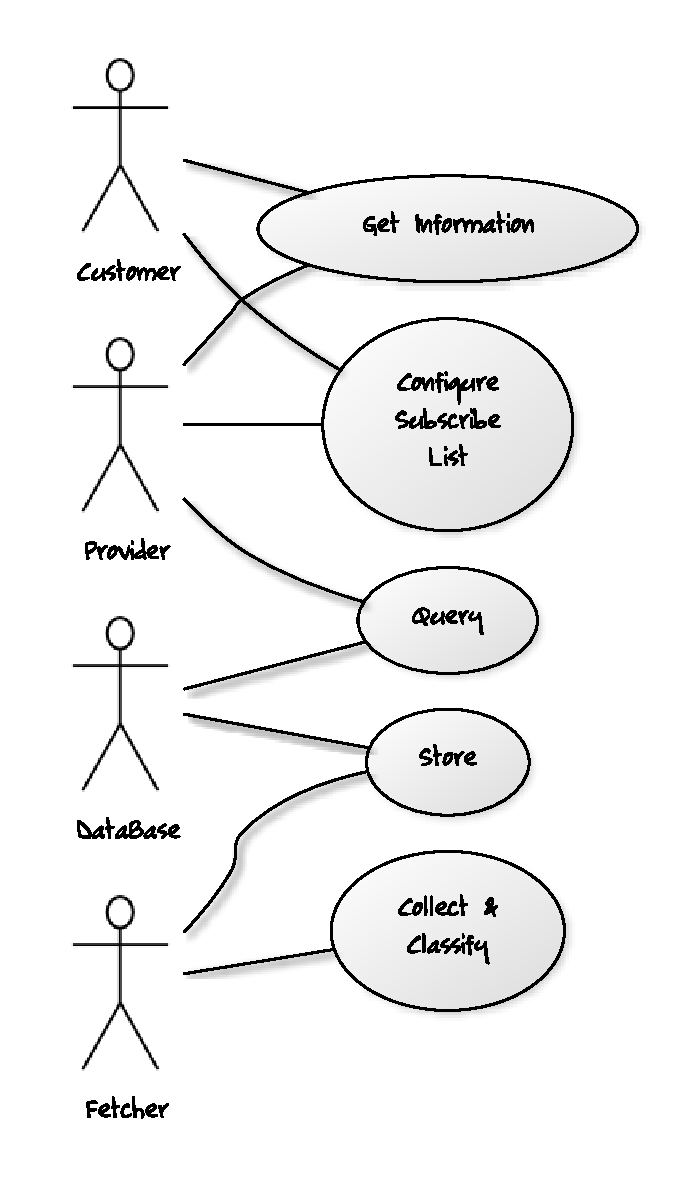
\includegraphics[]{./figure/basic}
  \caption{Basic User Case\label{user-case-diagram}}
  \end{figure}

\section{Priority}
  Features taged Core means it must be implemented. After them the work will focus on features from High to Low.
  \begin{center}
  \begin{table}[h]
    \begin{center}
    \begin{tabular}{c|c|c}
      Feature & Core & Priority \\ \hline
      Fetch Information & $\star$ & High \\
      Configure Subscribe List & $\star$ & High \\
      APIs & $\star$ & High \\
      Website &  & High \\
      Client Application &   & Middle \\
      Mobile Application &   & Low \\
      Internationalization &   & Low \\
    \end{tabular}
    \end{center}
    \caption{Priority}
  \end{table}
  \end{center}

\section{Timeline}
  The main work flow is like this.
  \begin{center}
  \begin{table}[h]
    \begin{center}
    \begin{tabular}{c|c|c}
      Progress & Start & Deadline \\ \hline
      Design & Sept. 25th & Oct. 12th \\
      Collection Prototype & Oct. 13th & Oct. 21st \\
      Classification Prototype & Oct. 13th & Oct. 21st \\
      Prototype Intergration & Oct. 16th & Oct. 25th \\
      Website & Oct. 16th & Oct. 31st \\
      Clients & TBD & TBD
    \end{tabular}
    \end{center}
    \caption{Timeline}
  \end{table}
  \end{center}

\section{Evaluation}
  In order to check whether this collector really works, these tests will be done.
  \subsection{Core}
    \begin{itemize}
      \item[]{Fetch articles from web portal and other website.}
      \item[]{Fetch private information of specific consumer.}
      \item[]{Configure subscribe list.}
    \end{itemize}
  \subsection{Website}
    \begin{itemize}
      \item[]{Friendly UI.}
      \item[]{Anti XSS, CSRF and SQL injection attack.}
    \end{itemize}
